\pretocmd{\chapter}{\glsresetall}{}{}

% Conclusion

% Main chapter title
%\chapter[toc version]{doc version}
\chapter{Conclusion}

% Short version of the title for the header
%\chaptermark{version for header}

% Chapter Label
% For referencing this chapter elsewhere, use \ref{ChapterTemplate}
\label{Conclusion}

The proposed approach presents a novel application of\ac{mcts} to\ac{ucttp}, combined with\ac{hc} for local improvements. While\ac{mcts} has seen limited application in\ac{ucttp}, this dissertation demonstrates its potential.

The integration of\ac{hc} significantly improves solution quality by exploiting feasible regions more effectively.

An additional innovation is the incorporation of a diving strategy into the\ac{mcts} process. This mechanism allows the algorithm to focus more deeply on promising branches of the search tree, accelerating convergence and reducing unnecessary exploration.

However, our findings indicate that both standard and diving-based\ac{mcts} tend to plateau after a certain number of iterations, with diminishing returns even under extended run times. While diving produces more consistent improvements and tends to stay closer to the best-found solutions, the problem of long-term stagnation remains and represents a key area for future optimization.

Our experimental results, including comparisons against the benchmark dataset from the ITC-2007 competition, show that the hybrid approach consistently produces feasible solutions. Although it does not yet outperform state-of-the-art solutions, this dissertation provides an effective and adaptive scheduling process for\ac{fcup} and can be extended to other institutions and help in other studies. 

\section{Future Work}

Future work may focus on fine tuning the algorithm, improving the heuristic functions, enhancing computational performance, and integrating a visualization tool.

\subsection{Performance}

One promising direction is to postpone room allocation during both tree construction and simulation. In this approach, the fixed nodes in the tree represent only the \((weekday, timeslot)\) (Appendix \ref{AppendixA} Figure \ref{fig:tree}) and, in the simulation, only allocate these two attributes for each event. Room assignments are performed afterward, once the simulation reaches a complete assignment of periods. Exploring this variant could help reduce computational overhead and allow a deeper or broader search within the same time constraints.

However, this approach might be less effective when the number of available rooms is limited. In such cases, delaying room assignments could lead to difficulties in finding feasible allocations later in the simulation.

Although early testing of this approach did not yield strong results, it remains a promising idea that deserves further investigation and refinement.

\subsection{Expand Hard and Soft Constraints}

Expanding the set of hard and soft constraints may also be important. For instance, additional hard constraints could enforce requirements such as assigning specific room types based on the nature of the class (e.g., labs requiring specialized equipment), while soft constraints could aim to give both lecturers and students a free period during lunchtime. Integrating such constraints would make the system more aligned with the practical needs and expectations of real-world academic environments.

\subsection{Visualization tool}

A previous project\footnote{\textbf{Front-end:} \url{https://github.com/luismdsleite/schedule} \textbf{Back-end:} \url{https://github.com/luismdsleite/schedule-backend}} developed a timetabling visualization tool using Flask and reactive programming principles with the Elm language. Flask facilitated data management and communication between the front-end and the database (Appendix \ref{AppendixA} Figure \ref{fig:previous_work_uml}), ensuring that timetable updates were efficiently processed and displayed. 

This tool allows users to manually construct and modify schedules while providing a responsive interface (Appendix \ref{AppendixA} Figure \ref{fig:previous_work_interface}). However, despite its usability, the tool has some limitations that this dissertation attempted to address:

\begin{itemize}
\item \textbf{No conflict detection support:} Users had to manually check for conflicts, increasing the risk of errors.
\item \textbf{Lack of automated guidance:} It did not provide recommendations or suggestions to help users make optimal scheduling decisions.
\item \textbf{No quality assessment:} The system lacked mechanisms to evaluate the quality of a given timetable.
\end{itemize}

The development process involved several adaptations and refinements. Initially, the previous work was analyzed and made functional, serving as a baseline for the new system. 

The\ac{mcts} algorithm was being developed while also being integrated into the front-end interface intended to showcase the project. However, as the focus shifted towards adapting it to the\ac{itc-2007} track 3 benchmark for performance evaluation and fine-tuning the algorithm, the front-end development gradually lost priority. As the algorithm evolved and diverged significantly from its original form, aligning it with the prior work proved difficult. Consequently, continuing its development would be time-consuming and ultimately not worthwhile, as it was primarily intended for demonstration purposes. Instead, the system should be directly integrated into the sigarra\footnote{\url{https://sigarra.up.pt/up/pt/web\_page.inicial}} website.

%\begin{figure}
%    \centering
%      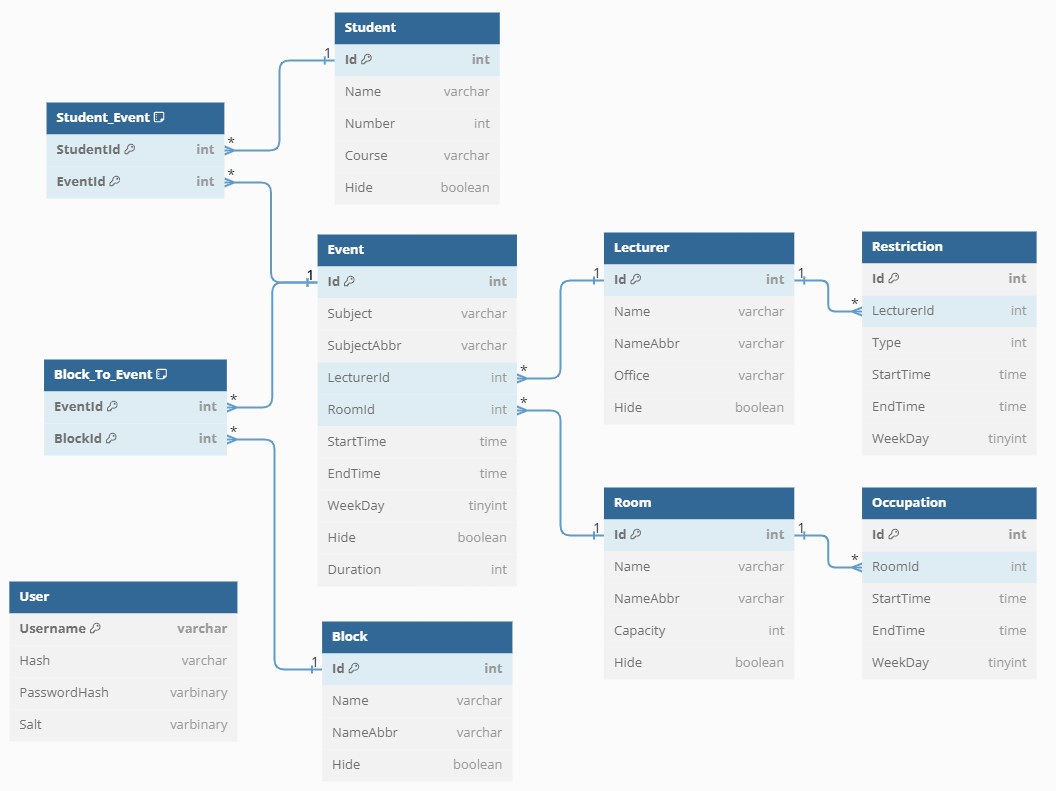
\includegraphics[width=1.1\columnwidth]{Development/uml.png}
%      \caption[UML]
%      {UML}
%      \label{fig:uml}
%\end{figure}


